% !TeX root = ../main.tex

% \begin{frame}
%   \frametitle{Relative Homology and The TCC}
%
%   \begin{itemize}
%     \item Relative homology and separation,
%     \item Properties of surrounding pairs,
%     \item Assumption 1 and The Geometric TCC,
%     \item Duality, Assumption 2, and the Algorithmic TCC.
%   \end{itemize}
% \end{frame}

\begin{frame}
  \frametitle{Relative Homology and Separation}

  % \begin{itemize}
  %   \item The idea of relative homology
  %   \item relative homology of separated sets
  % \end{itemize}

  \begin{textblock*}{10cm}(1cm,4.5cm)
    \centering
    \includegraphics<1,2>[width=\textwidth]{figures/h1_rel}
    \includegraphics<2>[width=\textwidth]{figures/h2_rel}
  \end{textblock*}

\end{frame}

\begin{frame}
  \frametitle{Properties of Surrounding Pairs}

  % \begin{itemize}
  %   \item surrounding pairs
  %   \item Coverage Lemma.
  %   \item Goal: show $\ell$ injective.
  % \end{itemize}

  % \only<1>{{\color{red} Handwave as a pseudo-boundary\\ Introduce idea of a sublevel set/points in a sublevelset as a boundary/sampled boundary}\\
  % \begin{definition}[Surrounding Pair]
  %   Let $X$ be a topological space and $(D,B)$ a pair in $X$.
  %   The set $B$ \textbf{surrounds $D$ in $X$} if $B$ separates $X$ with the pair $(D\setminus B, X\setminus D)$.
  %   We will refer to such a pair as a \textbf{surrounding pair in $X$}.
  % \end{definition}}
  \begin{textblock*}{11cm}(1cm,2cm)
    \only<1,2>{Function $f : D\to \R$\vspace{1ex}}

    \only<2>{Sample $P\subset D$ of $f$.}


    \only<3,4,5>{Sublevel set $B_\omega$ that \emph{surrounds} $D$.\vspace{1ex}}

    \only<4,5>{Sample $Q\subset P$ of $B_\omega$.}

    \only<6,7>{Would like to show that $Q^\delta$ surrounds $P^\delta$.\vspace{1ex}}

    \only<7>{Use \emph{surrounding pair} $(P^\delta, Q^\delta)$ to analyze $(D,B_\omega)$.}
  \end{textblock*}

  \begin{textblock*}{10cm}(1cm,5cm)
    \includegraphics<1>[trim=200 700 200 800, clip, width=0.6\textwidth]{../scripts/figures/partial2/full-surf}
    \includegraphics<2>[trim=200 700 200 800, clip, width=0.6\textwidth]{../scripts/figures/partial2/full-sample}
    \includegraphics<3>[trim=200 700 200 800, clip, width=0.6\textwidth]{../scripts/figures/partial2/topA-points}
    \includegraphics<4>[trim=200 700 200 800, clip, width=0.6\textwidth]{../scripts/figures/partial2/topB-points}
    % \includegraphics<5>[trim=200 700 200 800, clip, width=0.6\textwidth]{../scripts/figures/partial2/topB-cover}
    \includegraphics<5>[trim=200 700 200 800, clip, width=0.6\textwidth]{../scripts/figures/partial2/points_Q}
    \includegraphics<6>[trim=200 700 200 800, clip, width=0.6\textwidth]{../scripts/figures/partial2/cover_Q}
    \includegraphics<7>[trim=200 700 200 800, clip, width=0.6\textwidth]{../scripts/figures/partial2/cover}
  \end{textblock*}
\end{frame}

\begin{frame}
  \frametitle{Properties of Surrounding Pairs}

  % \begin{itemize}
  %   \item surrounding pairs
  %   \item Coverage Lemma.
  %   \item Goal: show $\ell$ injective.
  % \end{itemize}

  % \only<1>{{\color{red} Handwave as a pseudo-boundary\\ Introduce idea of a sublevel set/points in a sublevelset as a boundary/sampled boundary}\\
  % \begin{definition}[Surrounding Pair]
  %   Let $X$ be a topological space and $(D,B)$ a pair in $X$.
  %   The set $B$ \textbf{surrounds $D$ in $X$} if $B$ separates $X$ with the pair $(D\setminus B, X\setminus D)$.
  %   We will refer to such a pair as a \textbf{surrounding pair in $X$}.
  % \end{definition}}
  %
  % \only<2>{{\color{red} Picture of this}\\
  % \begin{small}\begin{lemma}\label{lem:coverage}
  %   Let $(D, B)$ be a surrounding pair in $X$ and $U\subseteq D$, $V\subseteq U\cap B$ be subsets.
  %   Let $\ell: \hom_0(X\setminus B, X\setminus D)\to \hom_0(X\setminus V, X\setminus U)$ be induced by inclusion.
  %   If $\ell$ is injective then $D\setminus B\subseteq U$ and $V$ surrounds $U$ in $D$.
  % \end{lemma}\end{small}}

  \begin{textblock*}{11cm}(1cm,2cm)\begin{small}
    % Surrounding pair $(D, B_\omega)$, $P^\delta\subseteq D$, $Q^\delta\subseteq B_\omega\cap P^\delta$.\vspace{2ex}

    $\ell : \hom_0(\overline{B_\omega}, \overline{D})\to \hom_0(\overline{Q^\delta}, \overline{P^\delta})$ induced by inclusion.\vspace{1ex}

    \only<2>{\begin{lemma}\label{lem:coverage}
      If $\ell$ is injective then $D\setminus B_\omega\subseteq P^\delta$ and $Q^\delta$ surrounds $P^\delta$ in $D$.
    \end{lemma}}
  \end{small}\end{textblock*}

  \begin{textblock*}{10cm}(1cm,5cm)
    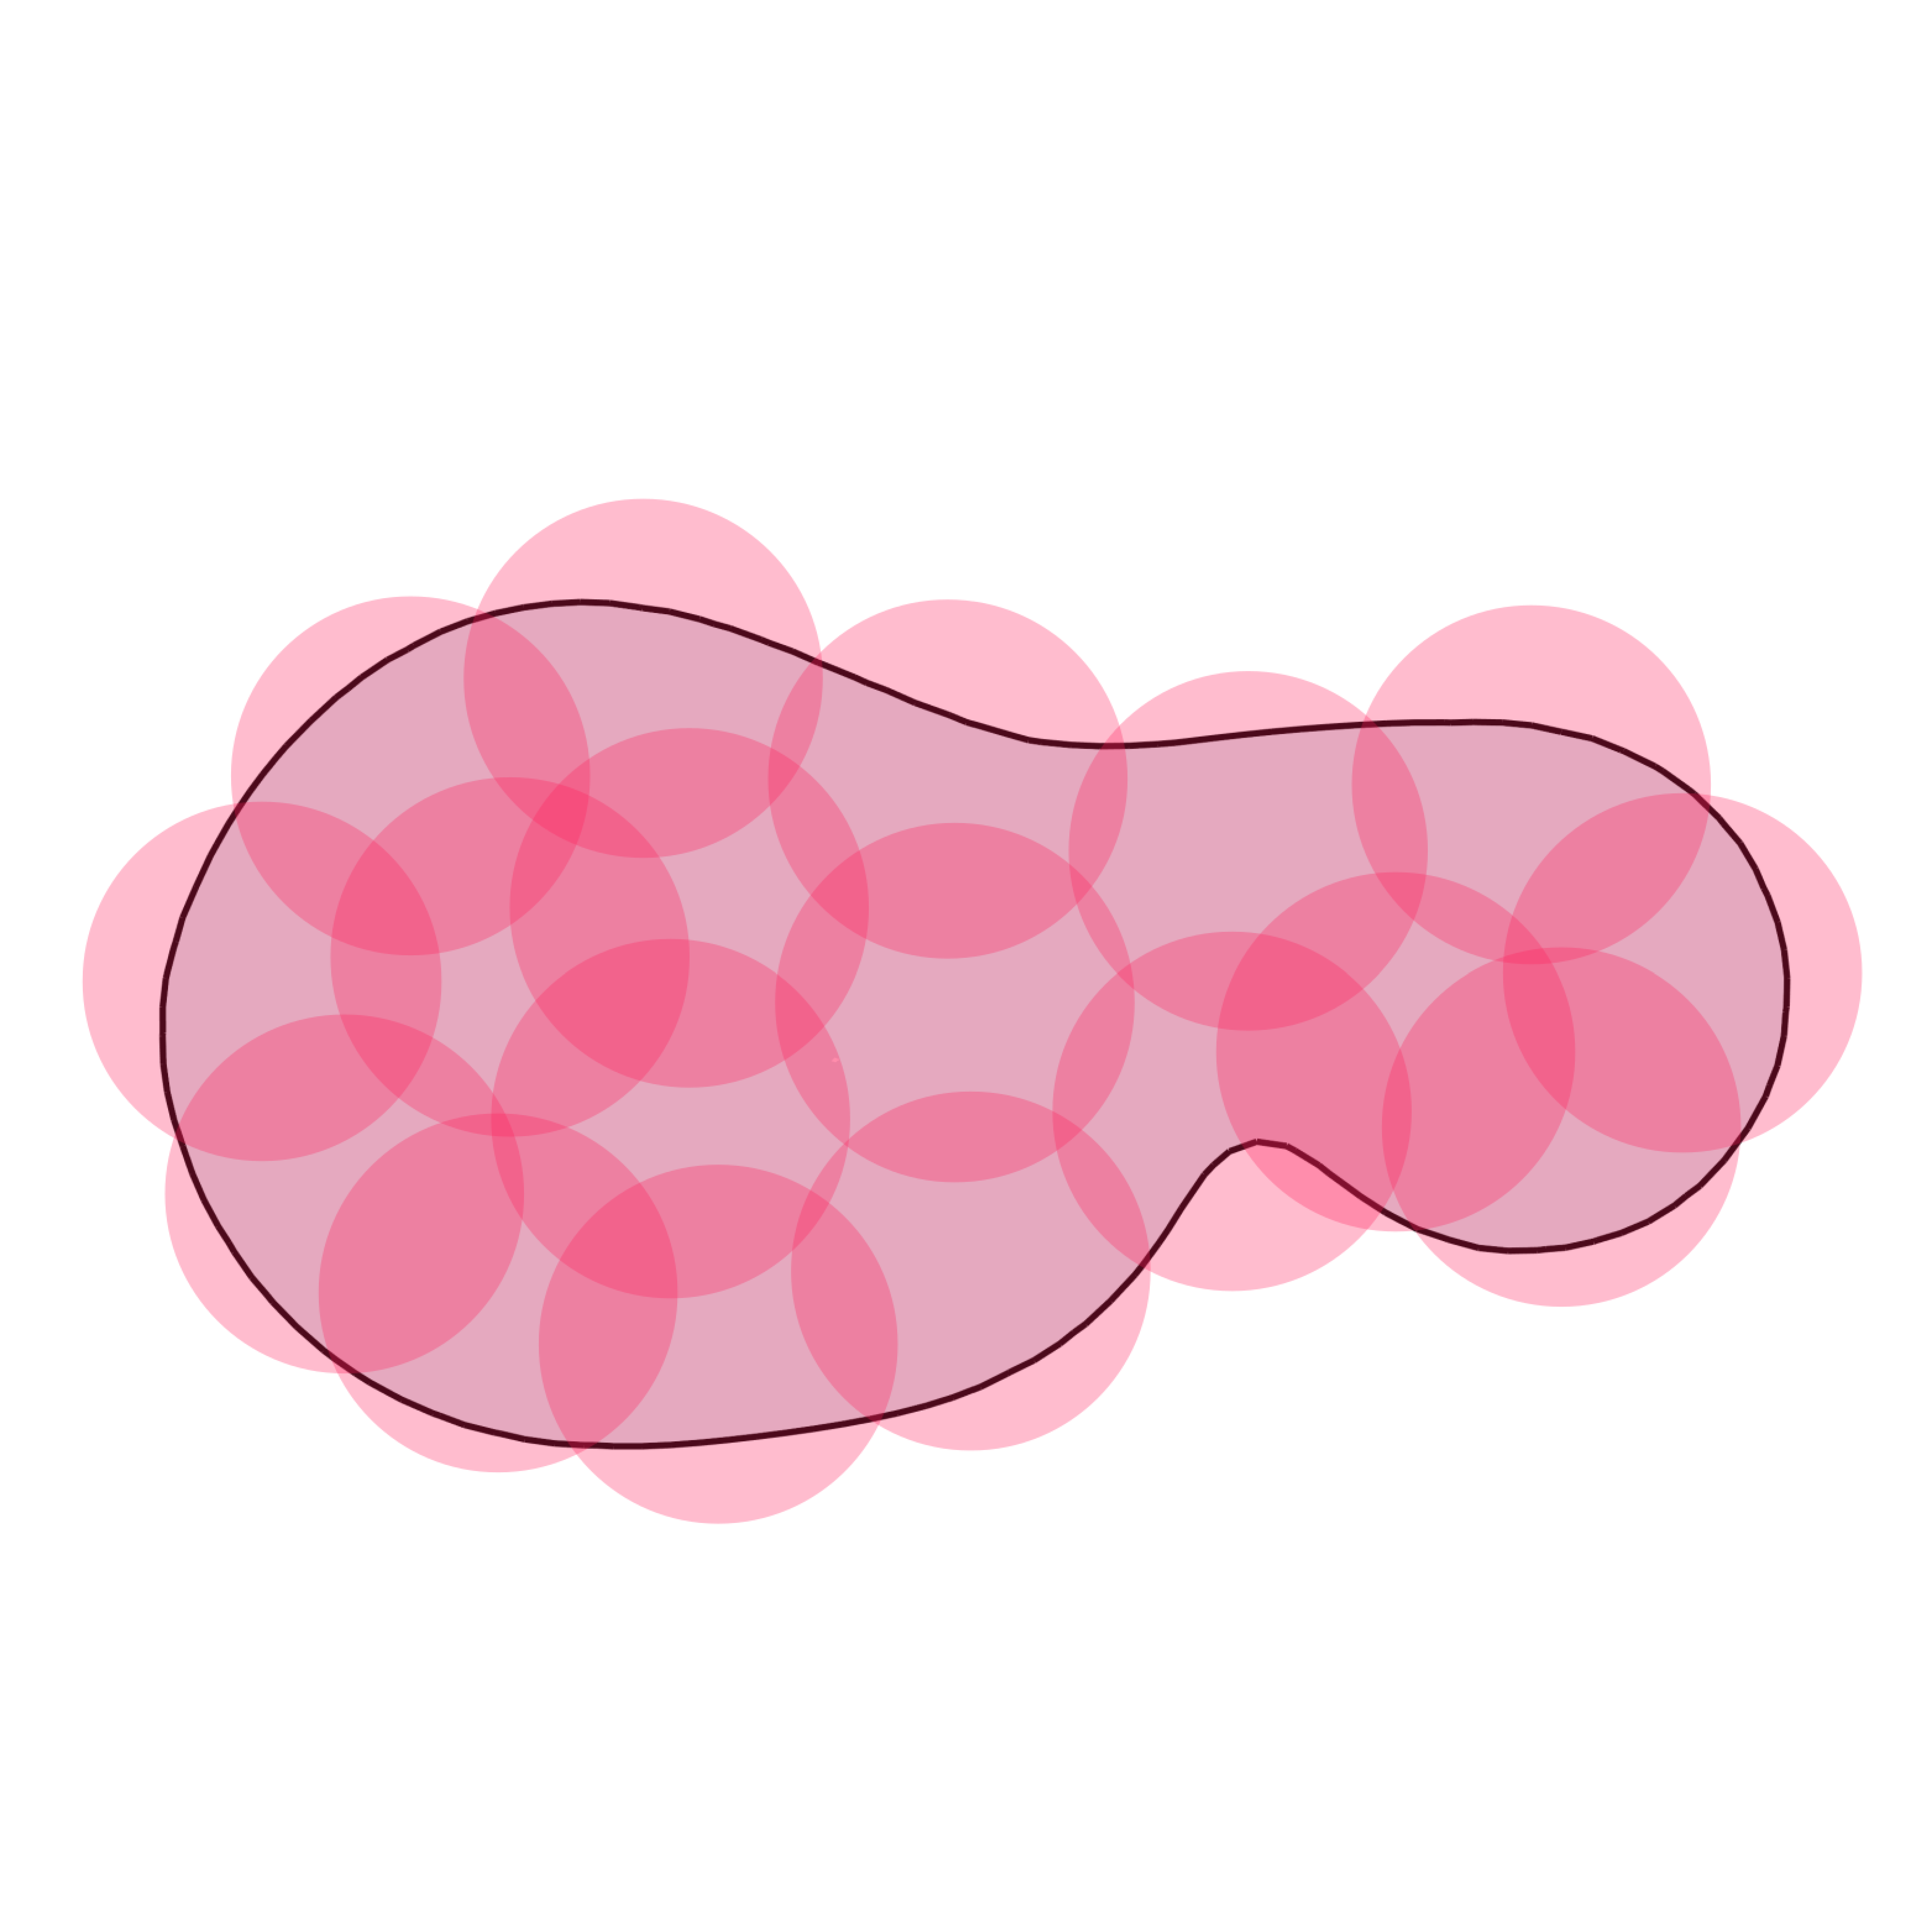
\includegraphics[trim=200 700 200 800, clip, width=0.6\textwidth]{../scripts/figures/partial2/cover}
  \end{textblock*}
\end{frame}

\begin{frame}
  % \frametitle{{\small Setup and Notation}}
  \frametitle{{\small Assumption 1 and the Geometric TCC}}

  \begin{textblock*}{11cm}(1cm,2cm)

    Constants $\zeta\geq\delta > 0$.\vspace{1ex}

    \only<2,3,4>{Let $Q_0 := P\cap B_{\omega-c\zeta}$ and $Q_1 := P\cap B_{\omega+c\delta}$.\vspace{1ex}}

    \only<3,4>{Let $i : \hom_0(\overline{Q_1^\delta}, \overline{P^\delta})\to \hom_0(\overline{Q_0^\delta}, \overline{P^\delta})$.}
  \end{textblock*}

  \begin{textblock*}{11cm}(1cm,5cm)
  \only<4>{
    \begin{lemma}\label{lem:psurj}
        If $B_\omega$ surrounds $D$ in $\X$ then $\mathbf{dim}~\hom_0(\overline{B_\omega}, \overline{D})\geq \mathbf{rk}~i$.
    \end{lemma}}
  \end{textblock*}

  % Compact $D\subset\X$, $c$-Lipschitz $f : D\to\R$.\\
  % % $\omega\in\R$ such that $\B := f^{-1}((-\infty, \omega])$ surrounds $D$ in $\X$.\\
  % $\omega\in\R$ such that $B_\omega$ surrounds $D$ in $\X$.\vspace{2ex}
  %
  % Finite $P\subset D$, $Q_\alpha := P\cap B_\alpha$ for $\alpha\in\R$.\\
  % Constants $\zeta\geq\delta > 0$.\vspace{2ex}
  %
  % {\color{red} some pictures to establish $Q_0, Q_1$}
\end{frame}

% \begin{frame}
%   \frametitle{Results Summary}
%
%   Quickly state both assumptions and theorems.
% \end{frame}

\begin{frame}
  \frametitle{{\small Assumption 1 and the Geometric TCC}}

  % \begin{equation}\label{dgm:1}
  % \begin{tikzcd}
  %   (P^\delta, Q_{\omega-c\zeta}^\delta) \arrow[hookrightarrow]{r}\arrow[hookrightarrow]{d} &
  %   (P^\delta, Q_{\omega+c\delta}^\delta) \arrow[hookrightarrow]{d} \\
  %   %
  %   (D, B_\omega) \arrow[hookrightarrow]{r} &
  %   (D, B_{\omega+c(\delta+\zeta)}),
  % \end{tikzcd}
  % \begin{tikzcd}
  %   \hom_0(\overline{B_{\omega+c(\delta+\zeta)}},\overline{D})\arrow{d}{m} \arrow{r}{j} &
  %   \hom_0(\overline{B_\omega}, \overline{D}) \arrow{d}{\ell} \\
  %   %
  %   \hom_0(\overline{Q_{\omega+c\delta}^\delta}, \overline{P^\delta}) \arrow{r}{i} &
  %   \hom_0(\overline{Q_{\omega-c\zeta}^\delta}, \overline{P^\delta}).
  % \end{tikzcd}\end{equation}
  \begin{textblock*}{11cm}(1cm,2cm)
    {\color{red} establish $B_1$}

    \textbf{Assumption 1}\\ $\hom_0(D\setminus B_{1}\hookrightarrow D\setminus B_\omega)$ is \emph{surjective}.
  \end{textblock*}

  \begin{textblock*}{11cm}(1cm,4.5cm)
    % 
\includegraphics[trim=50 190 0 200, clip, scale=0.2]{scripts/figures/scalar.png}
    % 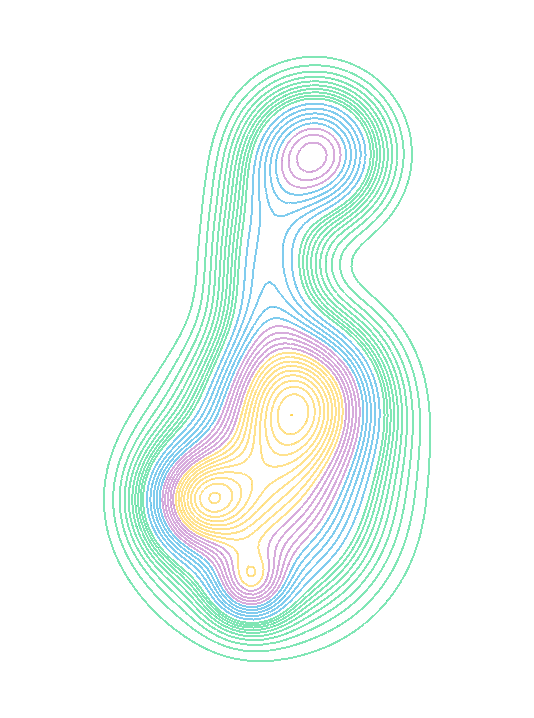
\includegraphics[trim=100 25 75 0, clip, angle=280, scale=0.25]{scripts/figures/scalar_contour.png}
    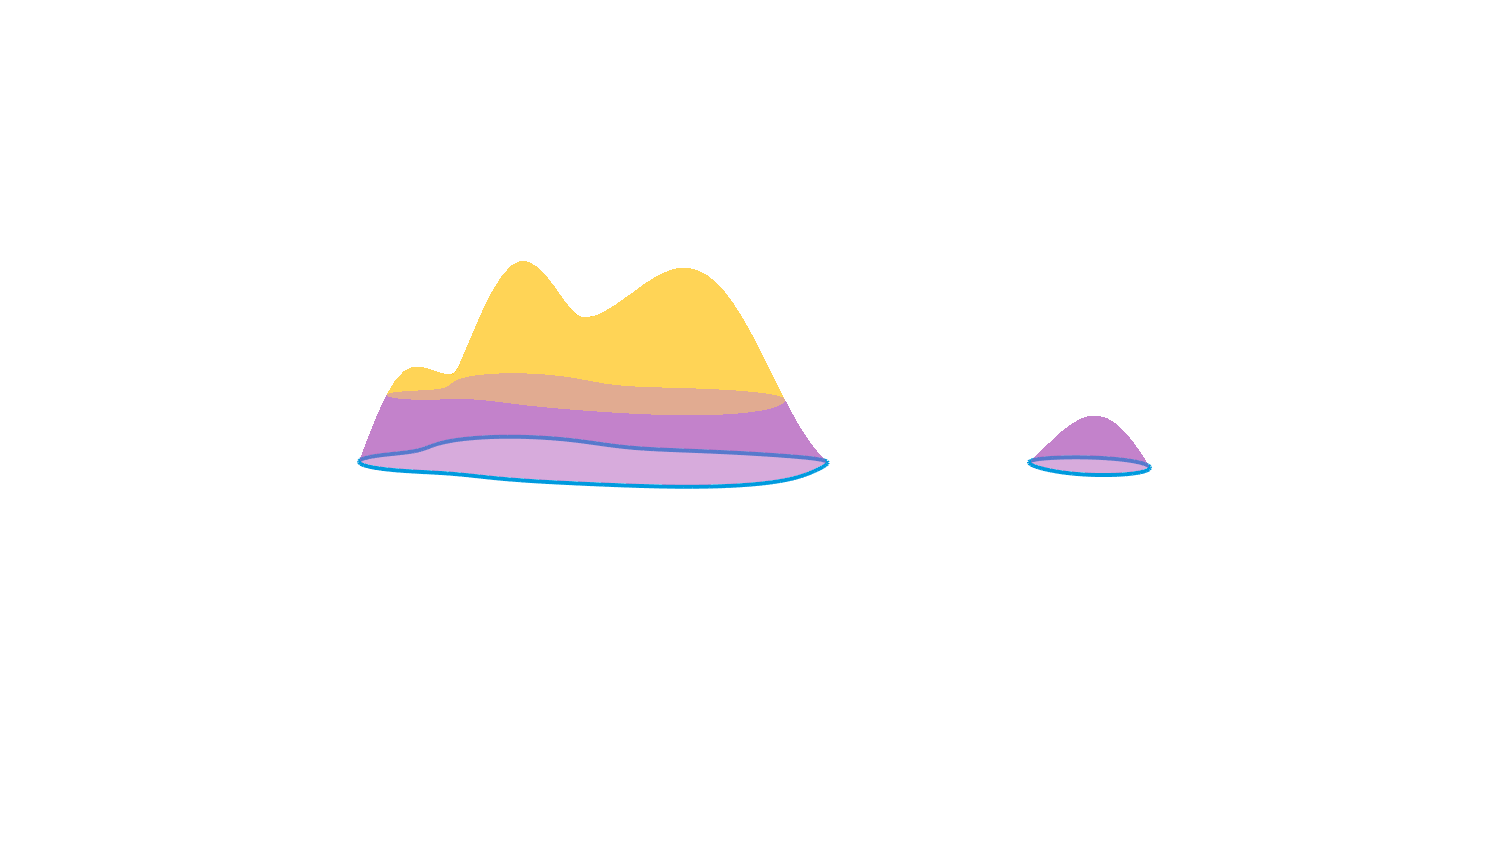
\includegraphics[trim=200 300 200 200, clip, width=0.5\textwidth]{../scripts/figures/surf/ass1_C_side.png}
    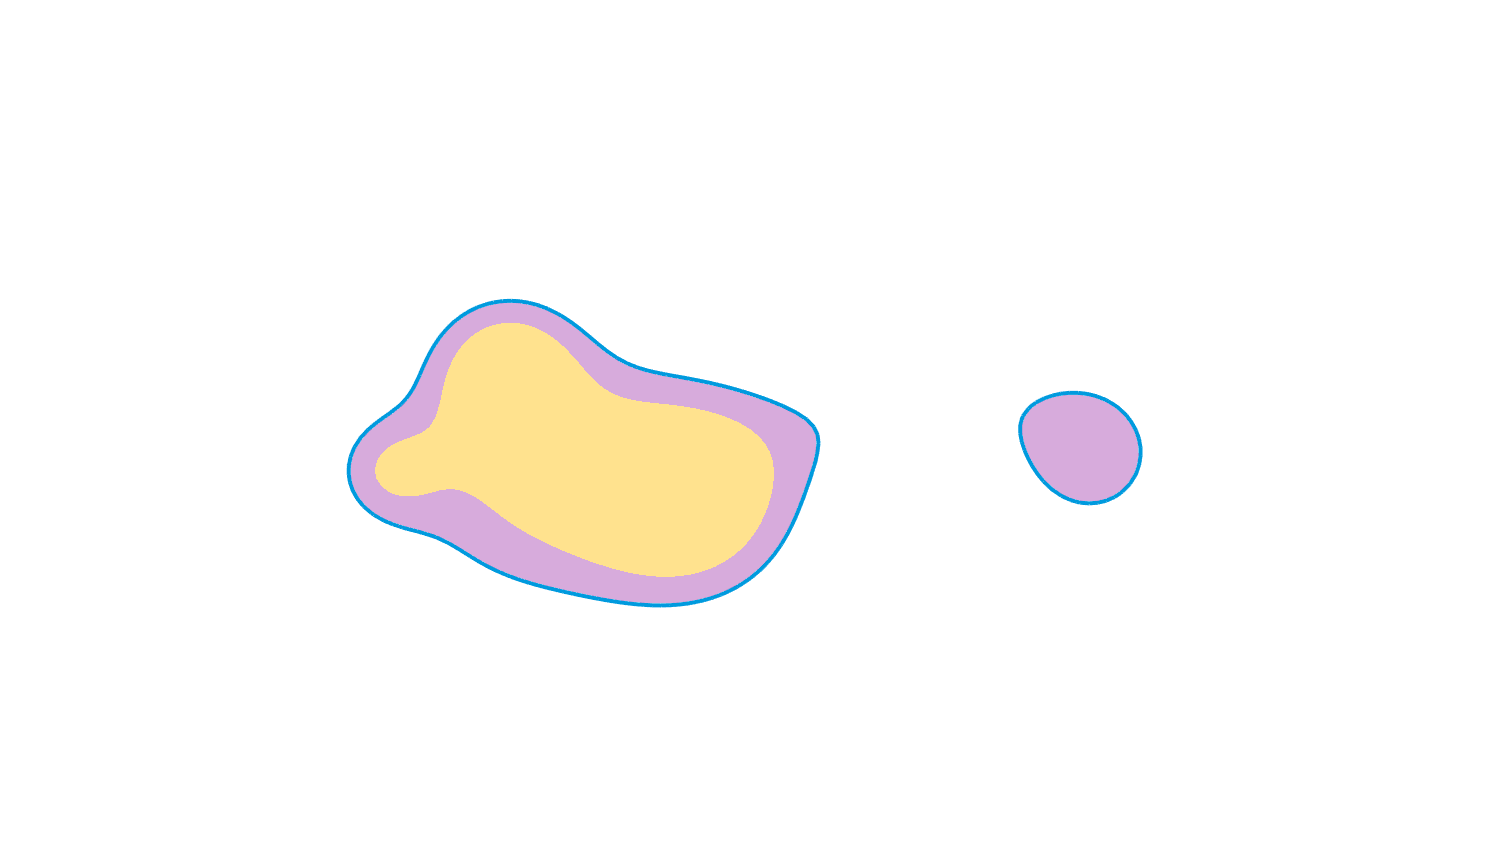
\includegraphics[trim=300 150 200 200, clip, width=0.3\textwidth]{../scripts/figures/surf/ass1_C_top.png}
    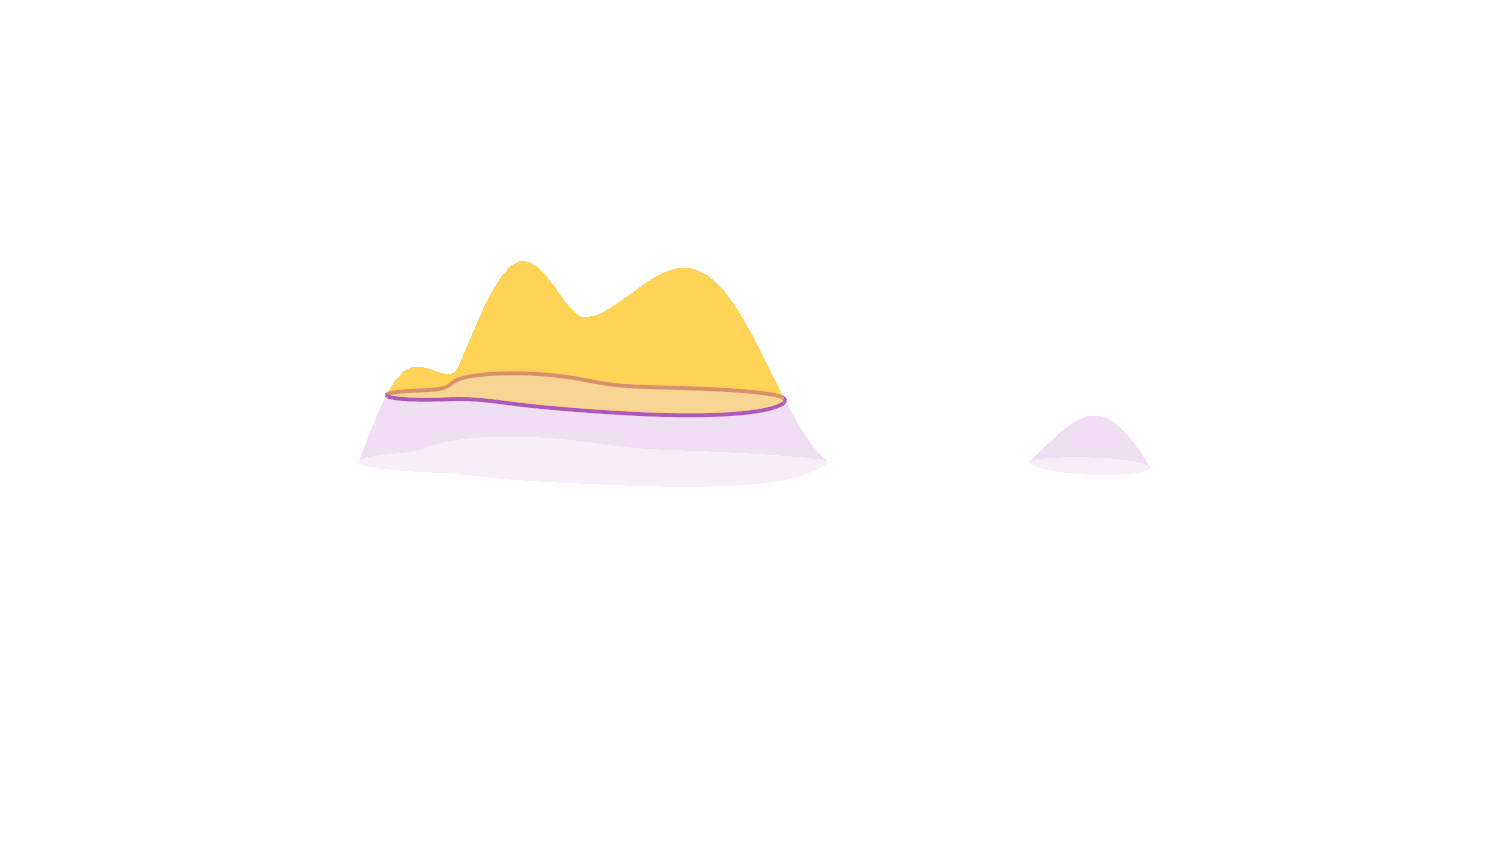
\includegraphics[trim=200 300 200 200, clip, width=0.5\textwidth]{../scripts/figures/surf/ass1_D_side.png}
    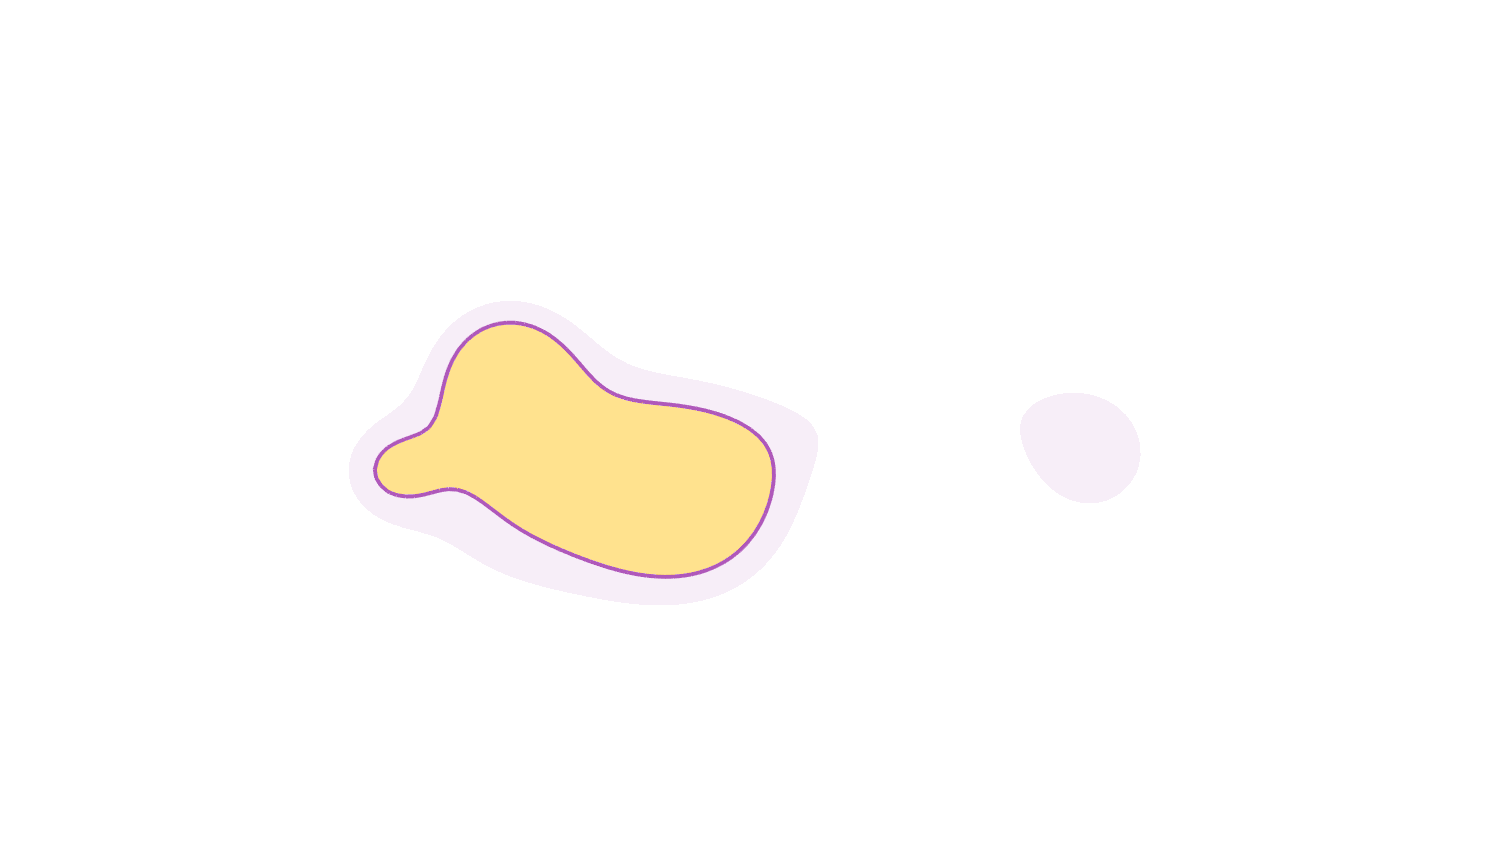
\includegraphics[trim=300 150 200 200, clip, width=0.3\textwidth]{../scripts/figures/surf/ass1_D_top.png}
    % 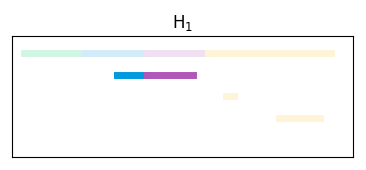
\includegraphics[scale=0.7]{scripts/figures/scalar_barcode_H1-masked.png}
  \end{textblock*}
\end{frame}

\begin{frame}
  \frametitle{{\small Assumption 1 and the Geometric TCC}}

  % \[\begin{tikzcd}
  %   \hom_0(\overline{B_{\omega+c(\delta+\zeta)}},\overline{D})\arrow{d}{m} \arrow{r}{j} &
  %   \hom_0(\overline{B_\omega}, \overline{D}) \arrow{d}{\ell} \\
  %   %
  %   \hom_0(\overline{Q_{\omega+c\delta}^\delta}, \overline{P^\delta}) \arrow{r}{i} &
  %   \hom_0(\overline{Q_{\omega-c\zeta}^\delta}, \overline{P^\delta}).
  % \end{tikzcd}\]

  \begin{theorem}[Geometric TCC]
    % Let $j : \hom_0(\cmp{B_{\omega+c(\delta+\zeta)}},\cmp{D})\to \hom_0(\cmp{\B},\cmp{D})$ and $i : \hom_0(\cmp{\QQ^\of}, \cmp{P^\of})\to \hom_0(\cmp{\Q^\of}, \cmp{P^\of})$ be induced by inclusion.
    %
    If $j$ is surjective and $\mathbf{rk}~i\geq \mathbf{rk}~j$ then $D\setminus B_\omega\subseteq P^\delta$ and $Q_{0}^\delta$ surrounds $P^\delta$ in $D$.
  \end{theorem}
\end{frame}

\begin{frame}
  \frametitle{{\small Duality, Assumption 2, and the Algorithmic TCC}}

  % \begin{itemize}
  %   \item Can't compute homology of complements: duality
  %   \item don't know number of connected components: assumption 2
  %   \item Rips-\v Cech interleaving and the Algorithmic TCC
  % \end{itemize}

  \textbf{Duality:} $\hom_d(P^\e,Q^\e)\cong\hom_0(D\setminus Q^\e, D\setminus P^\e)$.

  % \begin{textblock*}{12cm}(1cm,4.5cm)
  %
  % \end{textblock*}
\end{frame}


\begin{frame}
  \frametitle{{\small Duality, Assumption 2, and the Algorithmic TCC}}

  % \begin{itemize}
  %   \item Can't compute homology of complements: duality
  %   \item don't know number of connected components: assumption 2
  %   \item Rips-\v Cech interleaving and the Algorithmic TCC
  % \end{itemize}

  \only<1>{\begin{textblock*}{11cm}(1cm,2cm)
    \textbf{Assumption 2:} $\hom_0(D\setminus B_\omega\hookrightarrow D\setminus B_{0})$ is \emph{injective}.
  \end{textblock*}}

  \begin{textblock*}{12cm}(1cm,4.5cm)
    \includegraphics<1>[trim=200 300 200 200, clip, width=0.5\textwidth]{../scripts/figures/surf/ass2_C_side.png}
    \includegraphics<1>[trim=300 200 200 200, clip, width=0.3\textwidth]{../scripts/figures/surf/ass2_C_top.png}
    \includegraphics<1>[trim=200 300 200 200, clip, width=0.5\textwidth]{../scripts/figures/surf/ass2_B_side.png}
    \includegraphics<1>[trim=300 200 200 200, clip, width=0.3\textwidth]{../scripts/figures/surf/ass2_B_top.png}
  \end{textblock*}

  \only<2>{\begin{lemma}\label{lem:assumption2}
    If $\hom_0(D\setminus B_\omega\hookrightarrow D\setminus B_{1})$ is injective and each component of $D\setminus B_\omega$ contains a point in $P$ then $\mathbf{dim}~\hom_0(\rips^\delta(P\setminus Q_{0})) \geq \mathbf{dim}~\hom_0(D\setminus B_\omega)$.
  \end{lemma}}
\end{frame}

\begin{frame}
  \frametitle{{\small Duality, Assumption 2, and the Algorithmic TCC}}

  % \begin{itemize}
  %   \item Can't compute homology of complements: duality
  %   \item don't know number of connected components: assumption 2
  %   \item Rips-\v Cech interleaving and the Algorithmic TCC
  % \end{itemize}
  \begin{small}
    \[ \hom_k(\rips^\e(P, Q))\xrightarrow{J}\hom_k(\cech^\e(P, Q))\xrightarrow{I}\hom_k(\rips^\e(P, Q))\]
    % so
    % \[\mathbf{rk}~\hom_d(\cech^{\delta}(P, Q_{\omega-c\zeta})\hookrightarrow\cech^{\delta}(P, Q_{\omega+c\delta})) \geq\mathbf{rk}~ \hom_d(\rips^{\delta}(P, Q_{\omega-c\zeta})\hookrightarrow\rips^{2\delta}(P, Q_{\omega+c\delta}))\]

    % \begin{theorem}[Algorithmic TCC]\label{thm:algo_tcc}
    %   Suppose $\hom_0(D\setminus B_{\omega+c(\delta+\zeta)}\hookrightarrow D\setminus B_\omega)$ is surjective and $\hom_0(D\setminus B_\omega\hookrightarrow D\setminus B_{\omega-c(\delta+\zeta)})$ is injective.
    %
    %    If $\mathbf{rk}~\hom_d(\rips^\delta(P, Q_{\omega -c\zeta})\hookrightarrow \rips^{2\delta}(P, Q_{\omega+c\delta})) \geq \mathbf{dim}~\hom_0(\rips^\delta(P\setminus Q_{\omega-c\zeta}))$ then $D\setminus B_\omega\subseteq P^\delta$ and $Q_{\omega-c\zeta}^\delta$ surrounds $P^\delta$ in $D$.
    % \end{theorem}

    \begin{theorem}[Algorithmic TCC]\label{thm:algo_tcc}
      Suppose $\hom_0(D\setminus B_{1}\hookrightarrow D\setminus B_\omega)$ is surjective and $\hom_0(D\setminus B_\omega\hookrightarrow D\setminus B_{0})$ is injective.

       If $\mathbf{rk}~\hom_d(\rips^\delta(P, Q_{0})\hookrightarrow \rips^{2\delta}(P, Q_{1})) \geq \mathbf{dim}~\hom_0(\rips^\delta(P\setminus Q_{0}))$ then $D\setminus B_\omega\subseteq P^\delta$ and $Q_{0}^\delta$ surrounds $P^\delta$ in $D$.
    \end{theorem}
  \end{small}

  % \begin{textblock*}{12cm}(1cm,4.5cm)
  %
  % \end{textblock*}
\end{frame}
